\chapter{Opis części sprzętowej}
    %\section{Mikrokontroler Arduino Uno}

    

    \vspace{12pt}

    \begin{figure}[h!]
        \centering
        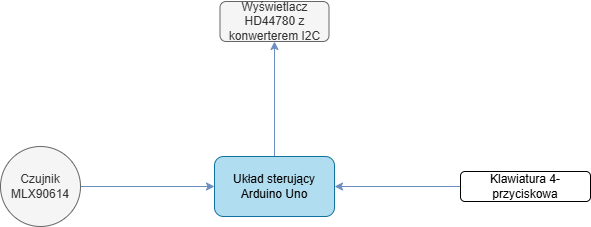
\includegraphics[width=1\textwidth]{images/schemat.png}
        \caption{Schemat blokowy skonstruowanego urządzenia} 
        \label{fig:schemat}
    \end{figure}

\section{Arduino Uno}

    Arduino Uno pokazany na rysunku \ref{fig:uno}, to popularny mikrokontroler wykorzystywany w projektach elektronicznych i robotyce. Jest to wszechstronna platforma programistyczna oparta na mikrokontrolerze ATmega328P. Mikrokontroler ten posiada 32KB pamięci Flash, 2KB pamięci RAM, 14 cyfrowych pinów wejścia/wyjścia, 6 pinów wejścia analogowego, zegar taktowany z częstotliwością 16MHz, interfejs USB, złącze zasilania 5V oraz złącze programowania ISP. Arduino Uno jest kompatybilny z wieloma dodatkowymi modułami, co pozwala na rozbudowę funkcjonalności. Mikrokontroler ten jest wykorzystywany w projekcie jako główny kontroler systemu \cite{5}.

    \vspace{12pt}

    Programowanie Arduino Uno odbywa się w dedykowanym środowisku Arduino IDE, które wykorzystuje język bazujący na C++. Dzięki rozbudowanej bibliotece funkcji i dużej społeczności użytkowników, realizacja nawet zaawansowanych projektów jest stosunkowo prosta.

    \vspace{12pt}

    \begin{figure}[h!]
        \centering
        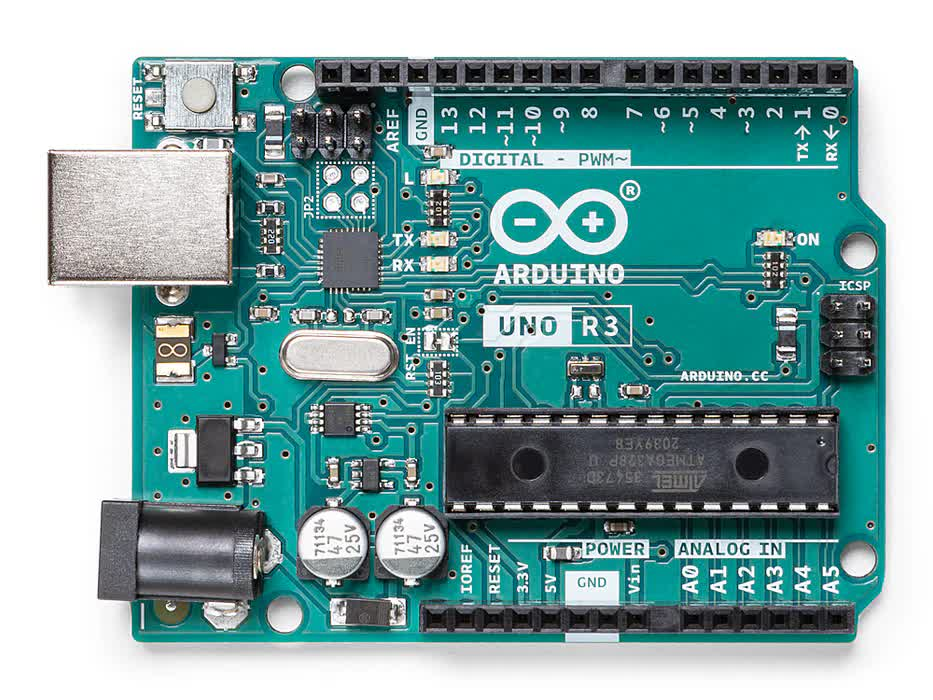
\includegraphics[width=0.45\textwidth]{images/uno.jpg}
        \caption{Mikrokontroler Arduino Uno \cite{5}}
        \label{fig:uno}
    \end{figure}

    \vspace{12pt}

\textbf{Zadanie:} Arduino Uno pełni funkcję jednostki centralnej systemu, integrując wszystkie kluczowe komponenty urządzenia. Jest odpowiedzialne za przetwarzanie danych pomiarowych z czujnika temperatury MLX90614, obsługę logiki systemu oraz sterowanie wyświetlaczem LCD. Dzięki temu użytkownik może w czasie rzeczywistym obserwować wyniki pomiarów i dokonywać ich konfiguracji za pomocą klawiatury. Arduino Uno zapewnia stabilne i niezawodne działanie, gwarantując synchronizację między komponentami. Ponadto, mikrokontroler umożliwia szybką reakcję na polecenia użytkownika, takie jak zmiana wartości emisyjności czy zmiana jednostek temperatury.

%\newpage

\vspace{12pt}

% \textbf{Specyfikacja:} Arduino Uno jest wyposażone w mikrokontroler ATmega328P, który posiada:
% \begin{itemize}
%     \item 14 cyfrowych pinów I/O (z możliwością generowania sygnałów PWM na 6 pinach),
%     \item 6 wejść analogowych do precyzyjnego odczytu sygnałów,
%     \item zegar o częstotliwości 16 MHz, zapewniający wystarczającą moc obliczeniową dla obsługi systemu,
%     \item 32 kB pamięci flash na kod programu, 2 kB SRAM na zmienne, oraz 1 kB EEPROM do przechowywania danych,
%     \item interfejsy komunikacyjne, takie jak UART, SPI, oraz I2C, co umożliwia łatwą integrację z czujnikami i innymi modułami,
%     \item zasilanie poprzez port USB (5V) lub zewnętrzne źródło zasilania (7-12V), co czyni go wszechstronnym w zastosowaniach przenośnych i stacjonarnych.
% \end{itemize}

\newpage

Dzięki swojej wszechstronności i otwartości Arduino Uno idealnie nadaje się do prototypowania urządzeń pomiarowych, takich jak projektowane w tym systemie rozwiązanie.


\vspace{12pt}

\section{Czujnik MLX90614}

    Czujnik MLX90614 pokazany na rysunku \ref{fig:mlx}, to zaawansowany, bezdotykowy termometr na podczerwień, który umożliwia pomiar temperatury obiektów w szerokim zakresie. Działa na napięciu zasilania od 3V do 3.6V i komunikuje się za pomocą interfejsu I2C, co czyni go łatwym w integracji z różnymi systemami, takimi jak Arduino czy inne mikrokontrolery. Dzięki swojej konstrukcji, MLX90614 znajduje zastosowanie w wielu dziedzinach, w tym w medycynie do pomiaru temperatury ciała, w systemach klimatyzacji oraz w automatyzacji przemysłowej \cite{6}.

    \begin{figure}[h!]
        \centering
        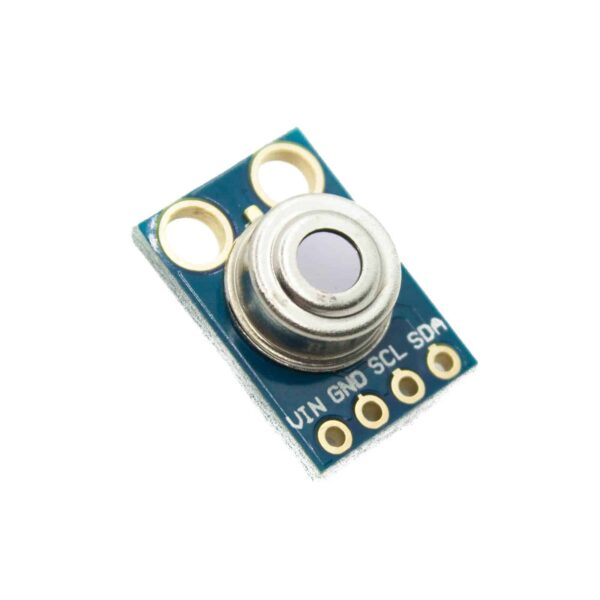
\includegraphics[width=0.38\textwidth]{images/mlx.jpg}
        \caption{Czujnik MLX90614 \cite{6}}
        \label{fig:mlx}
    \end{figure}

\textbf{Zadanie:} Czujnik MLX90614 stanowi kluczowy element systemu, umożliwiający precyzyjny, bezkontaktowy pomiar temperatury. Wykorzystuje technologię detekcji promieniowania podczerwonego, pozwalając na dokładny odczyt temperatury powierzchni bez konieczności fizycznego kontaktu z badanym obiektem.

\vspace{12pt}

%\textbf{Specyfikacja:} Zakres pomiaru od -70°C do 380°C, dokładność ±0.5°C, interfejs komunikacji I2C.

\vspace{12pt}

\section{Wyświetlacz LCD 16x2}

Wyświetlacz LCD z konwerterem I2C pokazany na rysnuku \ref{fig:lcd}, oparty jest na sterowniku HD44780 to popularne rozwiązanie do wyświetlania tekstu w projektach elektronicznych. Dzięki wbudowanemu konwerterowi I2C znacznie uproszczona jest komunikacja z mikrokontrolerem, ponieważ wymaga jedynie dwóch linii sygnałowych (SDA i SCL), zamiast standardowych 6-8 w przypadku klasycznego podłączenia. Wyświetlacz obsługuje różne konfiguracje, najczęściej spotykane to 16x2 (16 znaków na 2 liniach) lub 20x4 (20 znaków na 4 liniach) \cite{7}. Sterownik HD44780 umożliwia łatwe sterowanie wyświetlanymi znakami oraz tworzenie niestandardowych symboli. Dzięki czytelnemu interfejsowi i szerokiemu wsparciu w bibliotekach do Arduino, Raspberry Pi i innych platform, wyświetlacz ten jest chętnie używany w projektach takich jak panele kontrolne, wskaźniki statusu czy urządzenia IoT.

\begin{figure}[h!]
        \centering
        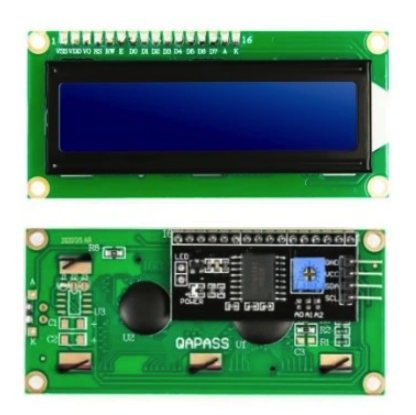
\includegraphics[width=0.45\textwidth]{images/lcd.png}
        \caption{Wyświetlacz LCD44780 z konwerterem I2C \cite{7}}
        \label{fig:lcd}
    \end{figure}

\textbf{Zadanie:} Wyświetlacz LCD 16x2 pełni funkcję interfejsu wizualnego, umożliwiając prezentację wyników pomiarów temperatury oraz dodatkowych informacji, takich jak ustawiona wartość emisyjności i wybrana jednostka temperatury (Celsjusz, Fahrenheit lub Kelvin).

\vspace{12pt}

%\textbf{Specyfikacja:} 16 kolumn i 2 wiersze znaków, kompatybilny z interfejsem HD44780, podświetlenie LED, kontrast sterowany potencjometrem na płycie.

\vspace{12pt}

\section{4-przyciskowa klawiatura}

Pokazana na zdjęciu \ref{fig:klaw}  klawiatura to membranowa klawiatura numeryczna, składająca się z czterech przycisków oznaczonych cyframi od 1 do 4. Charakteryzuje się prostą budową, elastyczną taśmą zakończoną złączem z pinami, co umożliwia łatwe podłączenie do mikrokontrolera lub innych urządzeń elektronicznych. Tego typu klawiatury są często wykorzystywane w prostych projektach elektronicznych, takich jak panele sterujące, systemy wprowadzania kodów czy interfejsy użytkownika w urządzeniach DIY. Dzięki niskiej cenie i kompaktowym rozmiarom, są popularnym wyborem wśród hobbystów i studentów elektroniki.

\begin{figure}[h!]
        \centering
        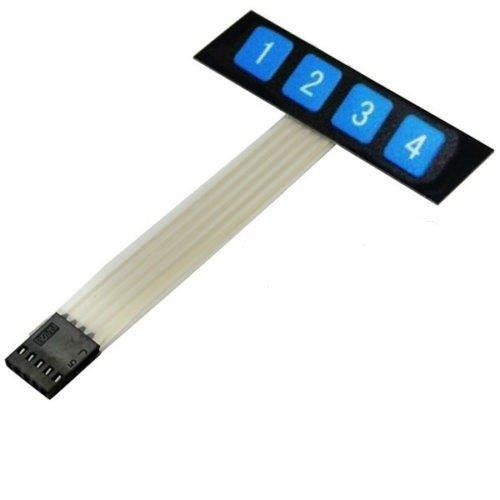
\includegraphics[width=0.35\textwidth]{images/keyboard4pin.jpg}
        \caption{4-przyciskowa klawiatura \cite{8}}
        \label{fig:klaw}
    \end{figure}

Za pomocą dołączonej 4-przyciskowej klawiatury można:
\begin{itemize}
    \item zwiększać wartość emisyjności,
    \item zmniejszać wartość emisyjności,
    \item przywrócić początkową wartość emisyjności wynoszącą 1,
    \item zmieniać jednostkę, w której wyświetlany jest wynik, wciskając kolejno przycisk (stopnie Celsjusza, Fahrenheita, Kelvina).
\end{itemize}

\textbf{Specyfikacja:} Prosty układ czterech przycisków, połączony z wejściami Arduino.

\vspace{12pt}

\section*{Rzeczywisty układ}

Na zdjęciu \ref{fig:panel_gorny} przedstawiono rzeczywiste wykonanie urządzenia, którego schemat blokowy zaprezentowano na rysunku \ref{fig:schemat}. Całość została zamontowana na płytce drukowanej i zabezpieczona przezroczystą osłoną, co zapewnia ochronę i wygodę obsługi.

\vspace{12pt}

Fotografia \ref{fig:panel_gorny} przedstawia panel górny urządzenia. Najważniejsze jego elementy:

\begin{enumerate}
    
    \item Czujnik MLX90614
    
    \item Układ sterujący Arduino Uno
    
    \item Wyświetlacz LCD HD44780 z konwerterem I2C
    
    \item Klawiatura 4-przyciskowa

\end{enumerate}

\begin{figure}[h!]
    \centering
    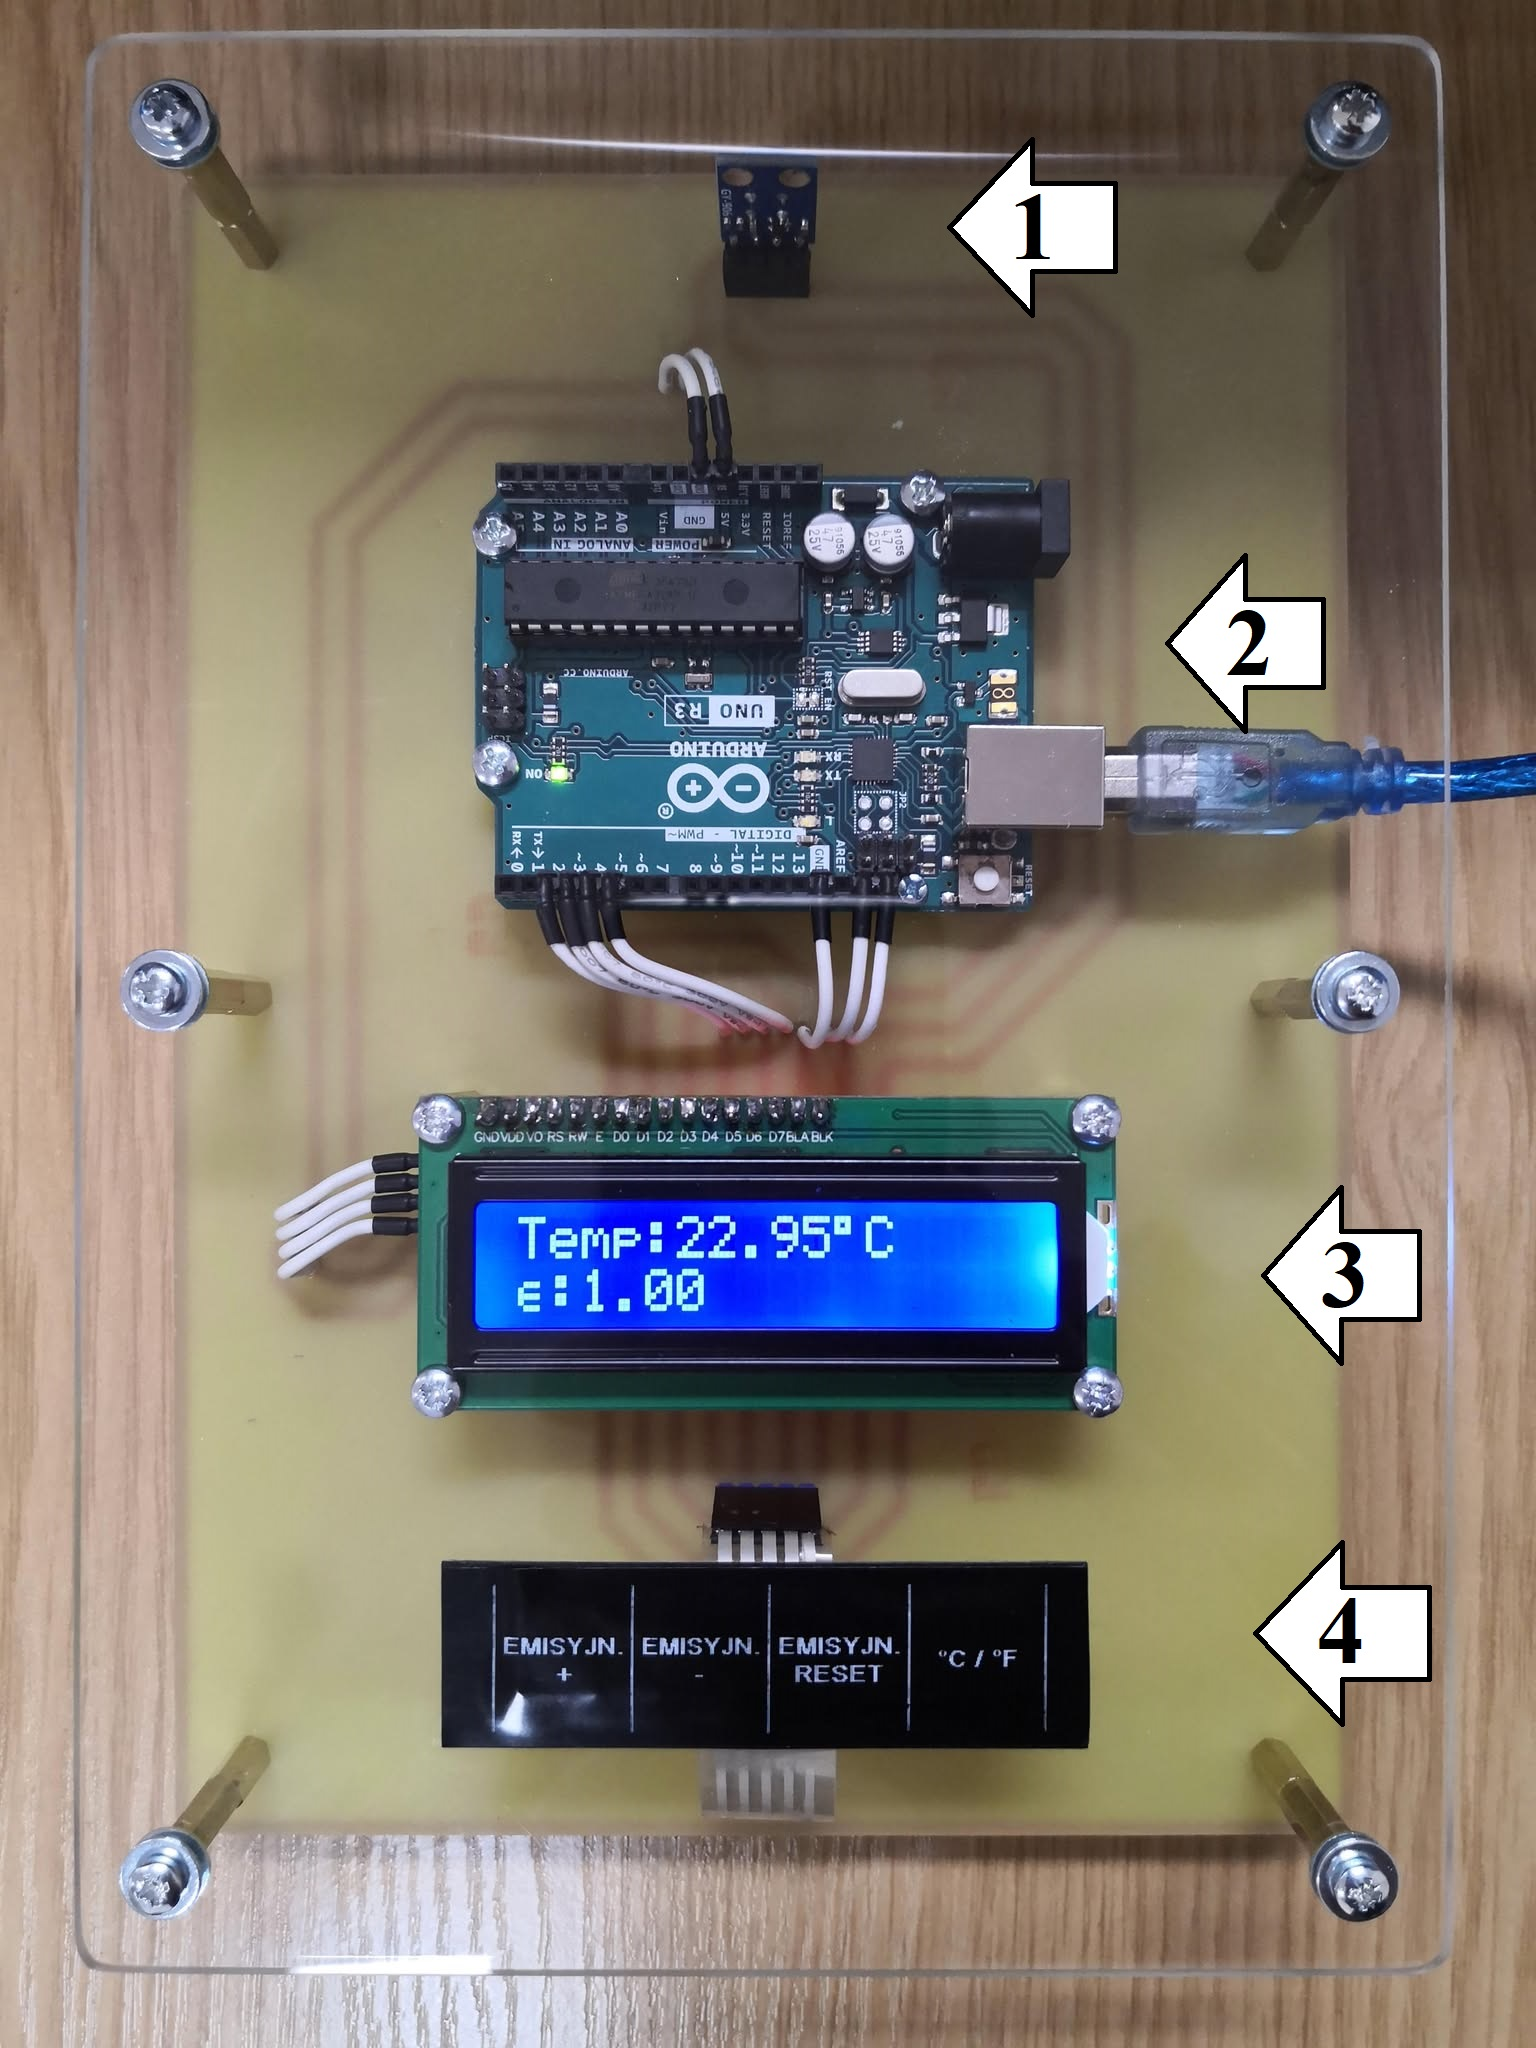
\includegraphics[width=0.595\textwidth]{images/front_opis.jpg}
   \caption{Panel górny urządzenia}
    \label{fig:panel_gorny}
\end{figure}

\section*{Część mechaniczna}

W oparciu o schemat \ref{fig:schemat} zaprojektowano specjalnie dostosowaną płytkę PCB, której schemat ideowy widoczny jest na rysunku \ref{fig:cad}, natomiast układ ścieżek na płytce drukowanej można dostrzeć na rysunku \ref{fig:pcb}. Łączy ona wszystkie podzespoły w jednej strukturze, gwarantując stabilność połączeń i zmniejszając ryzyko uszkodzeń obwodu. Dodatkowo pozwala na optymalne i przejrzyste rozmieszczenie elementów. Schemat przedstawiony na rysunku \ref{fig:cad} ilustruje sposób połączenia kluczowych komponentów urządzenia.  

\begin{itemize}
    \item \textbf{Arduino Uno} oznaczone jako U5
    \item \textbf{Czujnik MLX90614} oznaczony jako U1
    \item \textbf{Wyświetlacz LCD z interfejsem I2C} oznaczony jako U2 
    \item \textbf{Konwerter I2C dołączony do wyświetlacza} oznaczony jako U5 
    \item \textbf{Klawiatura 4-przyciskowa} oznaczona jako U3
\end{itemize}

\begin{figure}[h!]
    \centering
    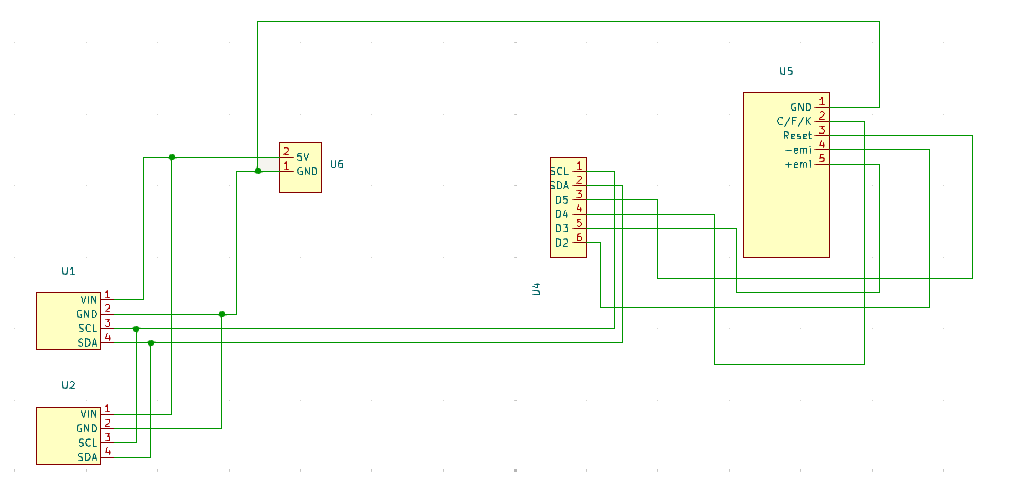
\includegraphics[width=1.1\textwidth]{images/cad.png}
    \caption{Schemat połączeń między komponentami}
    \label{fig:cad}
\end{figure}

Połączenia między elementami opierają się głównie na magistrali I2C oraz standardowych liniach sygnałowych, co minimalizuje liczbę przewodów i upraszcza konstrukcję układu.
Czujnik temperatury MLX90614 został podłączony do mikrokontrolera Arduino za pomocą interfejsu I2C. Wyświetlacz LCD HD44780 podłączono z wykorzystaniem konwertera pracującego na interfejsie I2C.% Do komunikacji z wyświetlaczem została użyta biblioteka LiquidCrystal\_I2C.h.

\vspace{12pt}

\section*{Płytka PCB}

Po przetestowaniu komponentów na płytce prototypowej, zaprojektowano docelową płytę ewaluacyjną z wykorzystaniem oprogramowania KiCad 8.0. Wykonano układ ścieżek na płytce drukowanej oraz rozmieszczono złącza w odpowiednich miejscach. Płyta ewaluacyjna definiuje rozmiar urządzenia, wynoszący 208 mm x 146 mm,
po dodaniu obudowy z płyty poliwęglanowej wysokość urządzenia ma wartość 46 mm.
Płytę ewaluacyjną wykonano z użyciem tradycyjnej technologii termotransferowej, a wytrawianie laminatu przebiegło z użyciem chlorku sodu. Po wykonaniu odpowiednich otworów w płycie, umieszczono złącza i przewody metodą lutowania THT. Wszystkie elementy urządzenia połączone zostały śrubami oraz tulejami mosiężnymi z gwintami w rozmiarze M3. Całość została obudowana dwiema płytami poliwęglanowymi o grubości 3 mm.

\begin{figure}[h!]
    \centering
    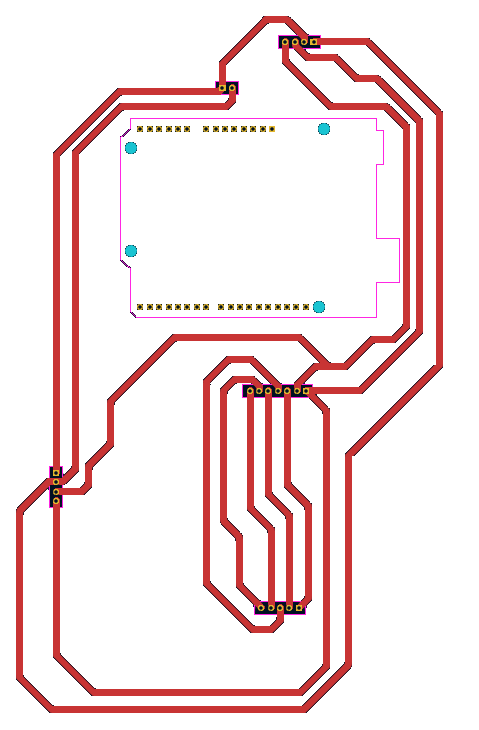
\includegraphics[width=0.8\textwidth]{images/layout.png}
    \caption{Rozkład ścieżek na płytce drukowanej}
    \label{fig:pcb}
\end{figure}

% \section{Zasilanie przez USB}
% \textbf{Rola:} System jest zasilany przez kabel USB podłączony do Arduino Uno, co upraszcza konstrukcję i eliminuje potrzebę stosowania zewnętrznych źródeł zasilania.

% \textbf{Specyfikacja:} Standardowy kabel USB do zasilania Arduino Uno, zapewniający napięcie 5V.

    % \begin{figure}[h!]
    %     \centering
    %     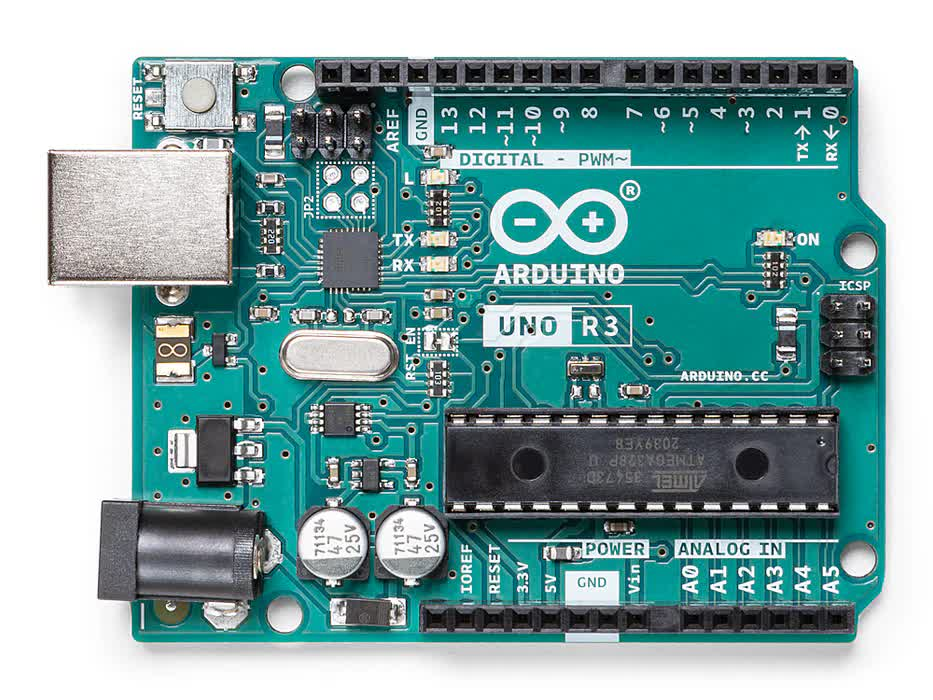
\includegraphics[width=0.32\textwidth]{images/uno.jpg}
    %     %\caption{Podpis pod obrazkiem.}
    %     \label{fig:example}
    % \end{figure}

    % Arduino Uno to popularny mikrokontroler wykorzystywany w projektach elektronicznych i robotyce. Jest to wszechstronna platforma programistyczna oparta na mikrokontrolerze ATmega328P. Mikrokontroler ten posiada 32KB pamięci Flash, 2KB pamięci RAM, 14 cyfrowych pinów wejścia/wyjścia, 6 pinów wejścia analogowego, zegar taktowany z częstotliwością 16MHz, interfejs USB, złącze zasilania 5V oraz złącze programowania ISP. Arduino Uno jest kompatybilny z wieloma dodatkowymi modułami, co pozwala na rozbudowę funkcjonalności. Mikrokontroler ten jest wykorzystywany w projekcie jako główny kontroler systemu.

    % \vspace{12pt}

    % Programowanie Arduino Uno odbywa się w dedykowanym środowisku Arduino IDE, które wykorzystuje język bazujący na C++. Dzięki rozbudowanej bibliotece funkcji i dużej społeczności użytkowników, realizacja nawet zaawansowanych projektów jest stosunkowo prosta \cite{4}
    
    % %\section{Czujnik temperatury MLX90614}

    % \begin{figure}[h!]
    %     \centering
    %     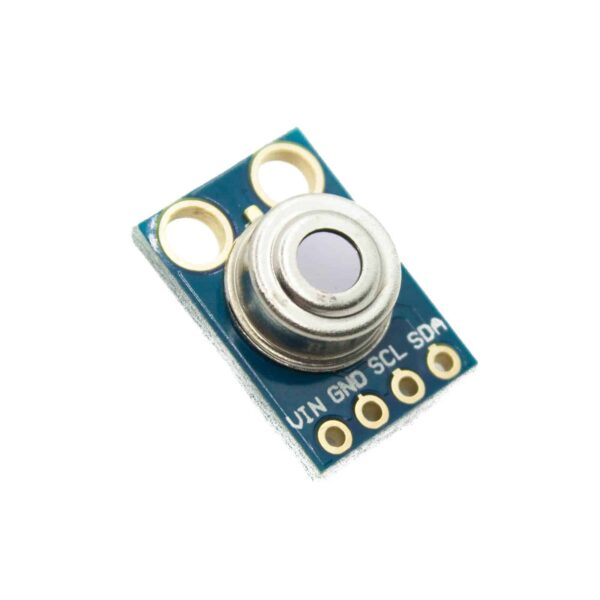
\includegraphics[width=0.32\textwidth]{images/mlx.jpg}
    %     %\caption{Podpis pod obrazkiem.}
    %     \label{fig:example}
    % \end{figure}

    % Czujnik MLX90614 to zaawansowany, bezdotykowy termometr na podczerwień, który umożliwia pomiar temperatury obiektów w szerokim zakresie. Działa na napięciu zasilania od 3V do 3.6V i komunikuje się za pomocą interfejsu I2C, co czyni go łatwym w integracji z różnymi systemami, takimi jak Arduino czy inne mikrokontrolery. Dzięki swojej konstrukcji, MLX90614 znajduje zastosowanie w wielu dziedzinach, w tym w medycynie do pomiaru temperatury ciała, w systemach klimatyzacji oraz w automatyzacji przemysłowej \cite{5}.

    % %\section{4-przyciskowa klawiatura}

    % \begin{figure}[h!]
    %     \centering
    %     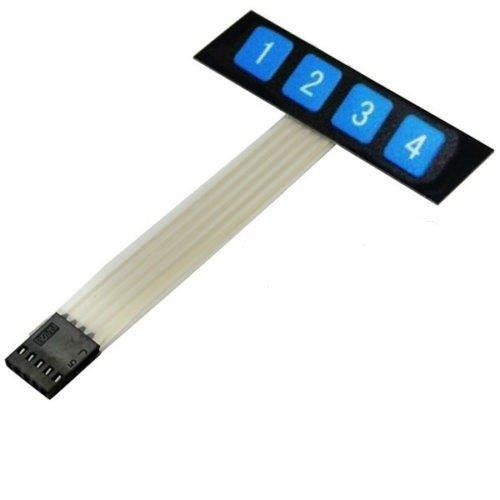
\includegraphics[width=0.32\textwidth]{images/keyboard4pin.jpg}
    %     %\caption{Podpis pod obrazkiem.}
    %     \label{fig:example}
    % \end{figure}

    % Pokazana na zdjęciu klawiatura to membranowa klawiatura numeryczna, składająca się z czterech przycisków oznaczonych cyframi od 1 do 4. Charakteryzuje się prostą budową, elastyczną taśmą zakończoną złączem z pinami, co umożliwia łatwe podłączenie do mikrokontrolera lub innych urządzeń elektronicznych. Tego typu klawiatury są często wykorzystywane w prostych projektach elektronicznych, takich jak panele sterujące, systemy wprowadzania kodów czy interfejsy użytkownika w urządzeniach DIY. Dzięki niskiej cenie i kompaktowym rozmiarom, są popularnym wyborem wśród hobbystów i studentów elektroniki.

    % %\section{Wyświetlacz LCD z konwerterem I2C HD44780}

    % \begin{figure}[h!]
    %     \centering
    %     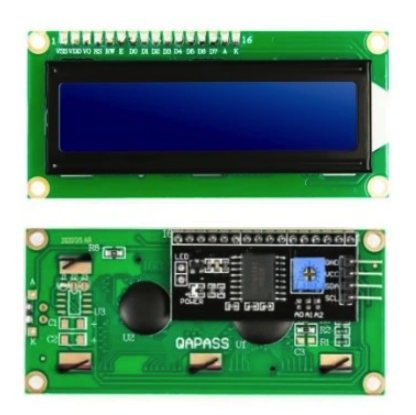
\includegraphics[width=0.3\textwidth]{images/lcd.png}
    %     %\caption{Podpis pod obrazkiem.}
    %     \label{fig:example}
    % \end{figure}
    
    % Wyświetlacz LCD z konwerterem I2C oparty na sterowniku HD44780 to popularne rozwiązanie do wyświetlania tekstu w projektach elektronicznych. Dzięki wbudowanemu konwerterowi I2C znacznie uproszczona jest komunikacja z mikrokontrolerem, ponieważ wymaga jedynie dwóch linii sygnałowych (SDA i SCL), zamiast standardowych 6-8 w przypadku klasycznego podłączenia. Wyświetlacz obsługuje różne konfiguracje, najczęściej spotykane to 16x2 (16 znaków na 2 liniach) lub 20x4 (20 znaków na 4 liniach). Sterownik HD44780 umożliwia łatwe sterowanie wyświetlanymi znakami oraz tworzenie niestandardowych symboli. Dzięki czytelnemu interfejsowi i szerokiemu wsparciu w bibliotekach do Arduino, Raspberry Pi i innych platform, wyświetlacz ten jest chętnie używany w projektach takich jak panele kontrolne, wskaźniki statusu czy urządzenia IoT.